\documentclass[12pt,a4paper]{article}
\usepackage{comment}
\usepackage[hidelinks]{hyperref}
\usepackage{listings}
\usepackage{graphicx}
\usepackage{subcaption}
\usepackage{float}
\usepackage[table,xcdraw]{xcolor}

\begin{comment}
    https://www.tablesgenerator.com/#
    We can create tables with this page so its easier to portray our examples
\end{comment}

\title{%
    \vspace*{-5mm}\Huge GW2-SRS TRANSFORM \\
    \vspace*{2mm}\Large powered by \LaTeX}

\author{\vspace*{-5mm}\large Daniel Lopez: \textbf{Transform algorithm}}

\begin{document}

    \maketitle

    \begin{figure}[H]
        \centering
        
\includegraphics[width=1 \textwidth]{Images/Nuevo_logo_GW2.png}
    \end{figure}

    \newpage

    \section*{2.0 TRANSFORM}

    \section*{\large 2.1 Introduction}
    After completing the data extraction, it was needed to do a deep cleaning on the files.
    The extracted data was displayed on the HTML source as a JSON type, it as well contained
    lots of information that is entirely related to the statistics in-game. Whether is true that
    statistics showed player names, player accounts, DPS\footnote{Damage Per Second}, etc. It
    also showed information that wasn't needed at all, where we could find EliteInsights information
    about it's version, release and EVTC\footnote{Unique log filetype from ArcDPS app} version as well.\\

    Therefore, I only wanted to gather clear stats data that could help me in the further
    analysis. The data I decided to aim for was:
    \begin{itemize}
        \item Player name
        \item Player Account
        \item Player Profession/Class
        \item Player DPS Statistics
    \end{itemize}

    \begin{table}[!h]
        \begin{tabular}{|c|llll}
        \hline
                                           & \multicolumn{1}{c|}{\cellcolor[HTML]{CBCEFB}Player's Name} & \multicolumn{1}{c|}{\cellcolor[HTML]{CBCEFB}Player's Account} & \multicolumn{1}{c|}{\cellcolor[HTML]{CBCEFB}Player's Class} & \multicolumn{1}{c|}{\cellcolor[HTML]{CBCEFB}Player's DPS} \\ \hline
        \cellcolor[HTML]{FFCCC9}\textbf{1} & \multicolumn{1}{c}{John\_Doe}                              & \multicolumn{1}{c}{johndoe.9752}                              & \multicolumn{1}{c}{Catalyst}                                & \multicolumn{1}{c}{35867.43}                              \\ \cline{1-1}
        \cellcolor[HTML]{FFCCC9}\textbf{2} & ...                                                        &                                                               &                                                             &                                                           \\ \cline{1-1}
        \cellcolor[HTML]{FFCCC9}\textbf{3} &                                                            &                                                               &                                                             &                                                           \\ \cline{1-1}
        \end{tabular}
    \end{table}

    \newpage

    \section*{\large 2.2 In-depth data explanation}
    In order to understand the data, I had to read and investigate the JSON files lots of times.
    Due to the JSON files size, I decided to use a JSON Viewer\footnote{http://jsonviewer.stack.hu/} 
    to help me with this task.\\

    \begin{figure}[h!]
        \centering
        \begin{subfigure}[b]{0.8\linewidth}
          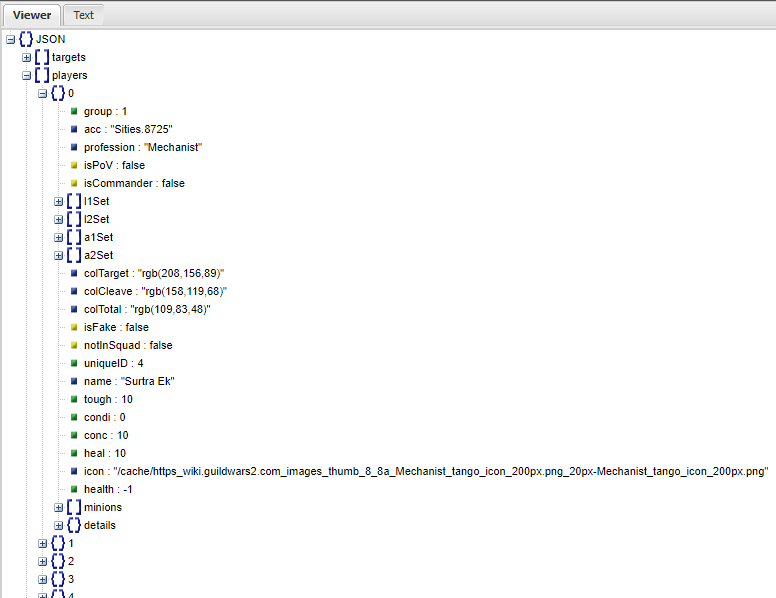
\includegraphics[width=\linewidth]{Images/json_schema.png}
          \caption{JSON Viewer formatted schema}
        \end{subfigure}

        \begin{subfigure}[b]{0.8\linewidth}
          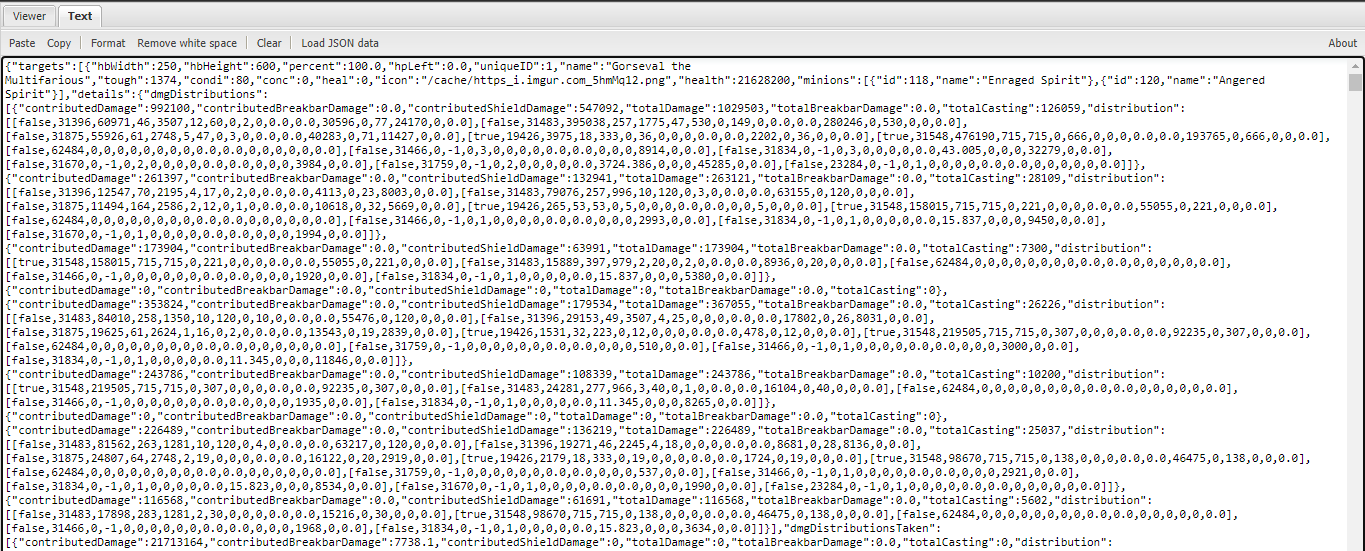
\includegraphics[width=\linewidth]{Images/json_raw.png}
          \caption{Raw JSON view}
        \end{subfigure}
    \end{figure}

    \newpage

    Using this method made the search of information extremely easy, for the most part, the essential
    player data like names, accounts and professions was pretty much finding each player and this data
    by it's index. I applied a zipped For loop to do the aggregation on SQL databases and on No-SQL databases
    I used a simple dictionary I created and then passed as a JSON dictionary.\\

    \begin{lstlisting}[language=Python, caption={\textbf{Basic player data loop}},captionpos=!b]
        for player in data['players']:
            player_group.append(player['group'])
            player_acc.append(player['acc'])
            player_names.append(player['name'])
            player_classes.append(player['profession'])
    \end{lstlisting}
    \begin{lstlisting}[language=Python, caption={\textbf{Custom Python stat dictionary}},captionpos=!b]
        stats_dict = {
                'boss': target,
                'players':{
                    'group': player_group,
                    'account': player_acc,
                    'names': player_names,
                    'profession': player_classes,
                    'phase_1_dps': player_dps1,
                    'phase_2_dps': player_dps2,
                    'phase_3_dps': player_dps3
                }
            }
    \end{lstlisting}
    
    \begin{lstlisting}[language=Python, caption={\textbf{Zipped data for SQLite query}},captionpos=!b]
        for (name,acc,profession) in zip \\
        (player_names,player_acc,player_classes):
    \end{lstlisting}

    It was important using a zipped For loop since the query need to be executed for every player.
    This is indeed not efficient if we look into the repetition of the same query for a simple operation
    but since there are only 10 players per boss fight, it ended up being rather useful.
\end{document}